\documentclass[a4paper,11pt]{article}

\usepackage{mlsubmit}

\begin{document}

\initmlsubmision{1}                              					% assignment number
								{Talla Aravind Reddy}      						           		% your name
								{14746}																		% your roll number

\begin{mlsolution}

\section*{Part 1}
Let $z=(x_1,y_1)$. We are given ${z_r}=(0,1)$ and ${z_g}=(1,0)$.
\\For the decision boundary, $d(z,z_r) = d(z,z_g)$ 
\\$\implies \langle z-z_r,U(z-z_r)\rangle = \langle z-z_g,U(z-z_g)\rangle $ 
where $U = \begin{bmatrix} 3 & 0  \\ 0 & 1 \end{bmatrix}$
\\$\implies 3x_1^2 + (y_1 - 1)^2 = 3(x_1 - 1)^2 + y_1^2 $
\\$\implies 3x_1^2 - 3(x_1 - 1)^2 =  y_1^2 - (y_1 - 1)^2$
\\$\implies 6x_1- 3 =  2y_1 - 1$
\\$\implies 3x_1 = y_1 + 1$
\\$\implies 3x = y+ 1$ is the decision boundary.

\section*{Part 2}
For the decision boundary, $d(z,z_r) = d(z,z_g)$ 
\\$\implies \langle z-z_r,U(z-z_r)\rangle = \langle z-z_g,U(z-z_g)\rangle $ 
where $U = \begin{bmatrix} 1 & 0  \\ 0 & 0 \end{bmatrix}$
\\$\implies x_1^2 = (x_1 - 1)^2$
\\$\implies 2x_1 - 1 =  0$
\\$\implies x_1 = \frac{1}{2}$
\\$\implies x = \frac{1}{2}$ is the decision boundary.

\begin{figure}[th]%
\centering
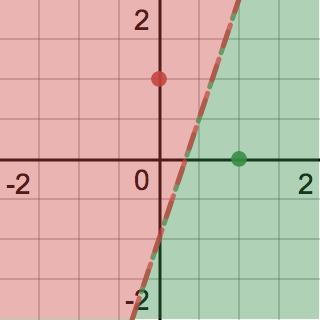
\includegraphics[width=0.3\columnwidth]{q1_graph1.png}%
\hfill
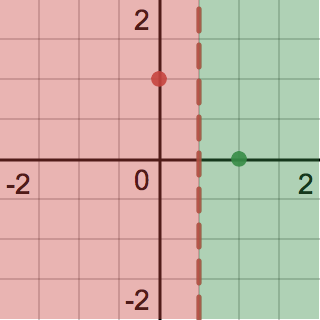
\includegraphics[width=0.3\columnwidth]{q1_graph2.png}%
\caption{The figure on the left shows the decision boundary for part 1 i.e $3x = y+ 1.$\newline The figure on the right shows the decision boundary for part 2 i.e $x = \frac{1}{2}$.}%
\label{fig:proto}%
\end{figure}

\end{mlsolution}

\begin{mlsolution}
One likelihood distribution which leads to $\mathbf{\hat{w}}_{cls}$ as the MAP estimate for the model is the gaussian distribution with mean as $\langle \mathbf{w,x}^i \rangle$ \[
\mathbb{P}[y|\mathbf{x}^i,w] = \mathcal{N}(\langle \mathbf{w,x}^i \rangle,\sigma^2) = \frac{1}{\sqrt{2\pi\sigma^2}} \text{exp}\bigg(-\frac{(y-\langle \mathbf{w,x}^i \rangle)^2}{2\sigma^2}\bigg)
\]
\\The prior distribution encapsulates the fact that $||\mathbf{w}||_2 \leq r$. This can be achieved by a uniform distribution over the $d$-dimensional ball with origin as centre and radius $r$.\[
\mathbb{P}[\mathbf{w}] = \mathcal{U}(\mathbf{0},r) = 
     \begin{cases}
       \cfrac{\Gamma(\frac{d}{2} + 1)}{\pi^{\frac{d}{2}} r^d} &\quad\text{if }||\mathbf{w}||_2 \leq r\\
       0 &\quad\text{if }||\mathbf{w}||_2 > r\\
     \end{cases}
\]

\end{mlsolution}

\begin{mlsolution}
The likelihood part of the estimate is same as the previous question, therefore one likelihood distribution is  the gaussian distribution with mean as $\langle \mathbf{w,x}^i \rangle$ \[
\mathbb{P}[y|\mathbf{x}^i,w] = \mathcal{N}(\langle \mathbf{w,x}^i \rangle,\sigma^2) = \frac{1}{\sqrt{2\pi\sigma^2}} \text{exp}\bigg(-\frac{(y-\langle \mathbf{w,x}^i \rangle)^2}{2\sigma^2}\bigg)
\]
For the prior, we can take a multivariate gaussian distribution with mean at $\mathbf{0}$\[
\mathbb{P}[\mathbf{w}] = \mathcal{N}(\mathbf{w};\mathbf{0},\Sigma) = \frac{1}{\sqrt{(2\pi)^d |\Sigma|}} \text{exp}\bigg(-\frac{1}{2}\mathbf{w}^T\Sigma^{-1}\mathbf{w}\bigg)
\]
Here $\Sigma = \sigma^2
\begin{bmatrix} 
\frac{1}{\alpha_1} & 0 & \dots & \dots & 0
\\ 0 & \frac{1}{\alpha_2} & 0 & \dots & 0
\\ \vdots & 0 & \ddots & 0\dots & 0
\\ \vdots & \vdots & \vdots & \frac{1}{\alpha_{d-1}} & 0
\\ 0 & 0 & 0 & 0 & \frac{1}{\alpha_d}
\end{bmatrix}$ i.e a diagonal matrix with it's $i$'th diagonal entry as $\frac{\sigma^2}{\alpha_i}$ where $\sigma^2$ is the variance of the likelihood distribution.\[
\text{log }\mathbb{P}[\mathbf{w|X,y}] = C -\frac{1}{2\sigma^2}\sum_{i=1}^{n}(y^i-\langle \mathbf{w,x}^i \rangle)^2 -\frac{1}{2\sigma^2}\sum_{j=1}^{d} \alpha_j \mathbf{w}_j^2 \]
\[ \implies \mathbf{\hat{w}}_{\text{MAP}} = \text{arg min} \sum_{i=1}^{n}(y^i-\langle \mathbf{w,x}^i \rangle)^2 + \sum_{j=1}^{d} \alpha_j \mathbf{w}_j^2   \]

\section*{Closed form expression:}
We need to minimise \[ \mathcal{L} =  \sum_{i=1}^{n}(y^i-\langle \mathbf{w,x}^i \rangle)^2 + \sum_{j=1}^{d} \alpha_j \mathbf{w}_j^2   \]
 \[ \mathcal{L} =  ||\mathbf{Xw - Y}||^2 + \sum_{j=1}^{d} \alpha_j \mathbf{w}_j^2   \]
 \[ \nabla_w \mathcal{L} = 2\mathbf{X}^T(\mathbf{Xw - Y}) + 2\mathbf{D_{\alpha}w} \text{ where } D_{\alpha} \text{ is the diagonal matrix with entries } \alpha_1,\alpha_2 \dots \alpha_d \]
 \[ \nabla_w \mathcal{L} = 2((\mathbf{X^T X + D_{\alpha})w} -\mathbf{X^T Y})\]
 \[\nabla_w \mathcal{L}= 0  \]
 \[ \iff (\mathbf{X^T X + D_{\alpha})w} -\mathbf{X^T Y} = 0 \]
 \[ \iff (\mathbf{X^T X + D_{\alpha})w}  = \mathbf{X^T Y} \]
 \[ \iff w = \mathbf{(X^T X + D_{\alpha})^{-1} X^T Y} \]
\end{mlsolution}

\begin{mlsolution}

\end{mlsolution}

\begin{mlsolution}
To prove: $\forall \mathbf{w'} \in \mathbb{R}^d, f(\mathbf{w'}) \geq f(\mathbf{w}) + \ip{\mathbf{g}}{\mathbf{w'-w}}$
\[
	f(\mathbf{w}) = \sum_{i=1}^{n}[1 - y^i \ip{\mathbf{w}}{\mathbf{x}^i}]_{+}
\]
where
\[
	[1 - y^i \ip{\mathbf{w}}{\mathbf{x}^i}]_{+} = 
     \begin{cases}
       1 - y^i \ip{\mathbf{w}}{\mathbf{x}^i} &\quad\text{if }y^i \ip{\mathbf{w}}{\mathbf{x}^i} < 1\\
       0 &\quad\text{if }y^i \ip{\mathbf{w}}{\mathbf{x}^i} \geq 1\\
     \end{cases}
\]

The given vector $\mathbf{g}$ is defined as $\mathbf{g} = \sum_{i=1}^{n}\mathbf{h}^i$ where 
\[
	\mathbf{h}^i = 
     \begin{cases}
      -y^i . \mathbf{x}^i  &\quad\text{if }y^i \ip{\mathbf{w}}{\mathbf{x}^i} < 1\\
       \mathbf{0}                          &\quad\text{if }y^i \ip{\mathbf{w}}{\mathbf{x}^i} \geq 1\\
     \end{cases}
\]
\[ f(\mathbf{w}) + \ip{\mathbf{g}}{\mathbf{w'-w}} = \sum_{i=1}^{n}[1 - y^i \ip{\mathbf{w}}{\mathbf{x}^i}]_{+} + \ip{\sum_{i=1}^{n}\mathbf{h}^i}{\mathbf{w'-w}} \]
\[ \implies f(\mathbf{w}) + \ip{\mathbf{g}}{\mathbf{w'-w}} = \sum_{i=1}^{n}[1 - y^i \ip{\mathbf{w}}{\mathbf{x}^i}]_{+} + \sum_{i=1}^{n}\ip{\mathbf{h}^i}{\mathbf{w'-w}} \]
\[ \implies f(\mathbf{w}) + \ip{\mathbf{g}}{\mathbf{w'-w}} = \sum_{i=1}^{n}\big([1 - y^i \ip{\mathbf{w}}{\mathbf{x}^i}]_{+} +\ip{\mathbf{h}^i}{\mathbf{w'-w}}\big) \]

For one value of $i$, we get four cases:
\\\underline{Case 1}: $y^i \ip{\mathbf{w}}{\mathbf{x}^i} < 1$, $y^i \ip{\mathbf{w'}}{\mathbf{x}^i} < 1$
\\In this case, the $i$'th term of $f(\mathbf{w}) + \ip{\mathbf{g}}{\mathbf{w'-w}}$ summation will be
\\ $1 - y^i \ip{\mathbf{w}}{\mathbf{x}^i} + \ip{\mathbf{h}^i}{\mathbf{w'-w}}  $
\\ $ = 1 - y^i \ip{\mathbf{w}}{\mathbf{x}^i} + \ip{-y^i . \mathbf{x}^i }{\mathbf{w'-w}}  $
\\ $ = 1 - y^i \ip{\mathbf{w}}{\mathbf{x}^i} +( -y^i) . \ip{\mathbf{x}^i }{\mathbf{w'-w}}  $
\\ $ = 1 - y^i \ip{\mathbf{w}}{\mathbf{x}^i} + (-y^i) . \ip{\mathbf{w'-w}}{\mathbf{x}^i}  $
\\ $ = 1 - y^i\big( \ip{\mathbf{w}}{\mathbf{x}^i} + \ip{\mathbf{w'-w}}{\mathbf{x}^i}\big)  $
\\ $ = 1 - y^i\ip{\mathbf{w+w'-w}}{\mathbf{x}^i}$
\\ $ = 1 - y^i\ip{\mathbf{w'}}{\mathbf{x}^i} $
\\This is the same as the $i$'th term of $f(\mathbf{w'})$ summation.\newline\newline
\underline{Case 2}: $y^i \ip{\mathbf{w}}{\mathbf{x}^i} < 1$, $y^i \ip{\mathbf{w'}}{\mathbf{x}^i} \geq 1$
\\In this case, the $i$'th term of $f(\mathbf{w}) + \ip{\mathbf{g}}{\mathbf{w'-w}}$ summation will be
\\ $1 - y^i \ip{\mathbf{w}}{\mathbf{x}^i} + \ip{\mathbf{h}^i}{\mathbf{w'-w}}  $
\\ $ = 1 - y^i \ip{\mathbf{w}}{\mathbf{x}^i} + \ip{-y^i . \mathbf{x}^i }{\mathbf{w'-w}}  $
\\ $ = 1 - y^i\ip{\mathbf{w'}}{\mathbf{x}^i} $
\\This is the same as the $i$'th term of $f(\mathbf{w'})$ summation.\newline\newline
\underline{Case 3}: $y^i \ip{\mathbf{w}}{\mathbf{x}^i} \geq 1$, $y^i \ip{\mathbf{w'}}{\mathbf{x}^i} < 1$
\\In this case, the $i$'th term of $f(\mathbf{w}) + \ip{\mathbf{g}}{\mathbf{w'-w}}$ summation will be
\\ $0 + \ip{\mathbf{0}}{\mathbf{w'-w}}  $
\\ $ = 0$
\\This is the less than the $i$'th term of $f(\mathbf{w'})$ summation i.e $1 - y^i \ip{\mathbf{w'}}{\mathbf{x}^i}$ .\newline\newline
\underline{Case 4}: $y^i \ip{\mathbf{w}}{\mathbf{x}^i} \geq 1$, $y^i \ip{\mathbf{w'}}{\mathbf{x}^i} \geq 1$
\\In this case, the $i$'th term of $f(\mathbf{w}) + \ip{\mathbf{g}}{\mathbf{w'-w}}$ summation will be
\\ $0 + \ip{\mathbf{0}}{\mathbf{w'-w}}  $
\\ $ = 0$
\\This is the same as the $i$'th term of $f(\mathbf{w'})$ summation.
\\ Thus in 3 of the 4 cases, the terms on LHS and RHS are equal.
\\ For the case 3, LHS is strictly greater than RHS.
\\Therefore, $\forall \mathbf{w'} \in \mathbb{R}^d, f(\mathbf{w'}) \geq f(\mathbf{w}) + \ip{\mathbf{g}}{\mathbf{w'-w}}$



\end{mlsolution}



\begin{mlsolution}
\section*{Part 1}
\begin{center}
\begin{tabular}{ |c|c|c| } 
 \hline
 $k$ & Test Error(\#points) \\ \hline
 1 & 4816 \\ 
 2 & 4288 \\
 3 & 3839 \\
 5 & 3542 \\
 10 & 3359 \\ 
 \hline
\end{tabular}
\end{center}

\begin{figure}[th]%
\centering
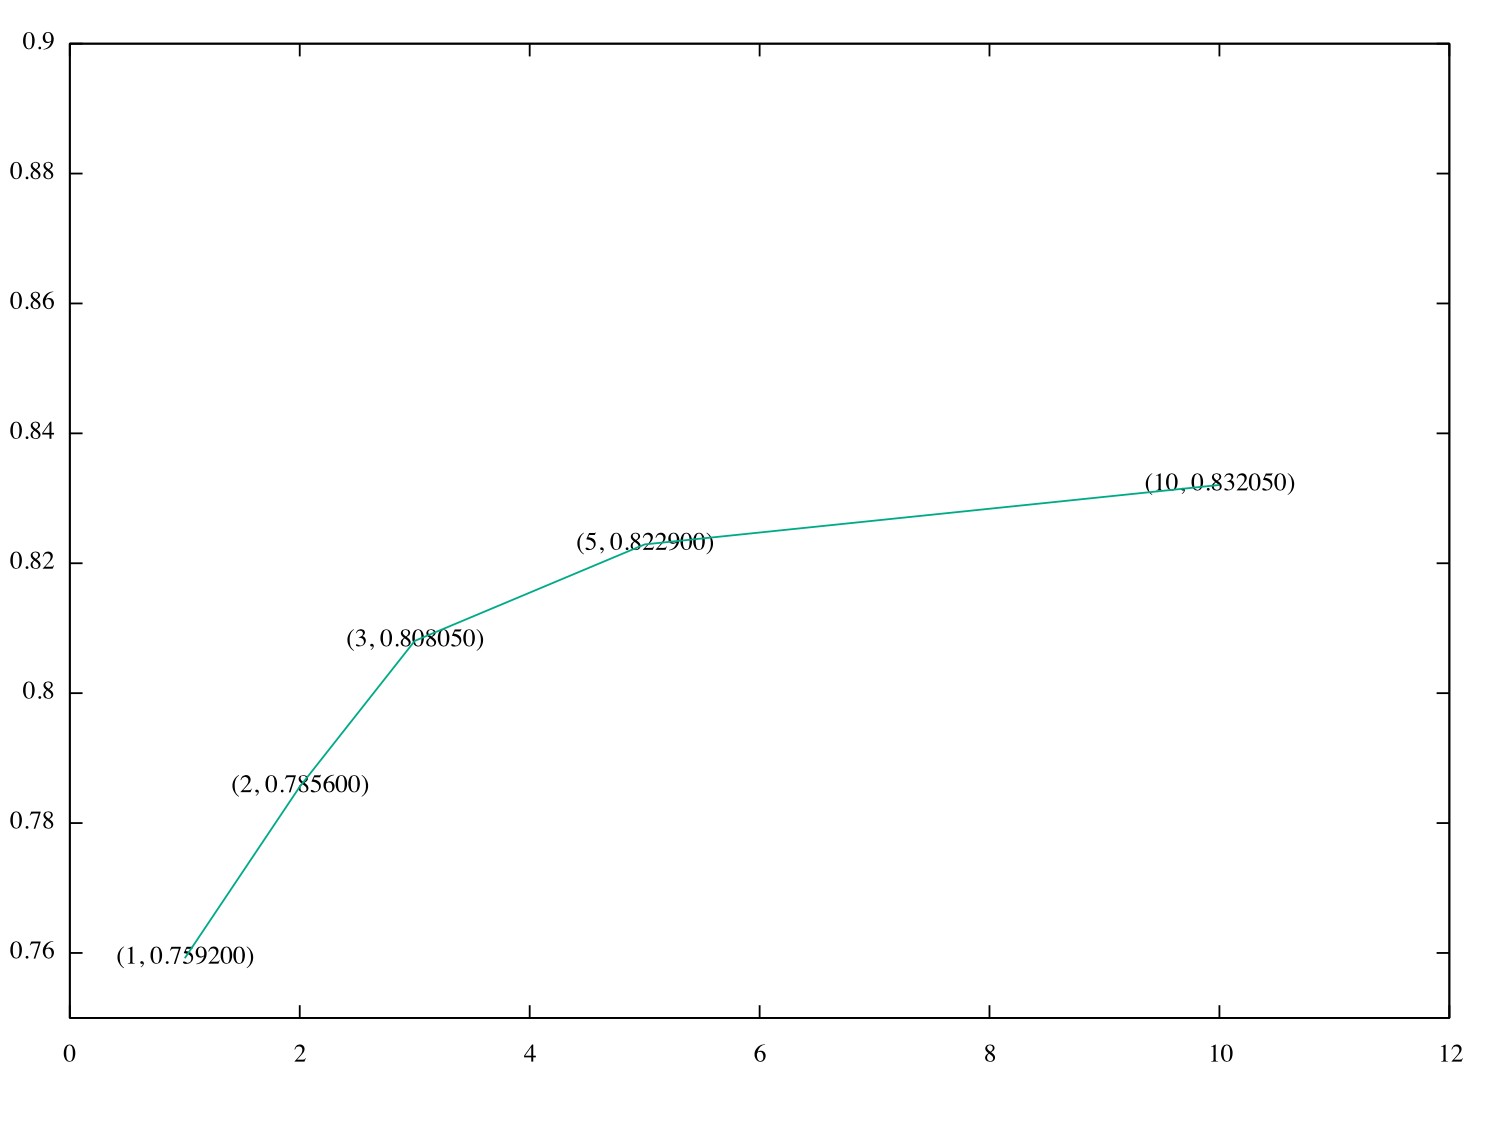
\includegraphics[scale = 0.5]{q61_plot.png}%
\label{fig:proto}%
\end{figure}

For lower values of $k$, the model overfits the training data. Therefore, due to the noise in the training data, the model has lesser accuracy for smaller values of $k$.

\section*{Part 2}
I used holdout validation for tuning the value of the hyperparameter $k$. I did a random shuffle of the given data of 60K points and took the first 50K points as the training set and the next 10K points as the validation set. We can see from the graph that there is not much change between the values from k=10 to k=20. Therefore, I took the value of k=10 for faster computation although k=16(the maxima) gives slightly better performance.

\begin{center}
\begin{tabular}{ |c|c|c|c|c|c|c|c| } 
 \hline
 $k$ & Accuracy & $k$ & Accuracy & $k$ & Accuracy & $k$ & Accuracy\\ \hline
 1 & 0.7631 & 2 & 0.7842 & 3 & 0.8060 & 4 & 0.8119 \\ 
 5 & 0.8183 & 6 & 0.8208 & 7 & 0.8224 & 8 & 0.8222 \\
 9 & 0.8244 & 10 & 0.8263 & 11 & 0.8255 & 12 & 0.8252 \\
 13 & 0.8258 & 14 & 0.8264 & 15 & 0.8262 & 16 & 0.8272\\
 17 & 0.8268 & 18 & 0.8257 & 19 & 0.8265 & 20 & 0.8252 \\ 
 \hline
\end{tabular}
\end{center}

\begin{figure}[th]%
\centering
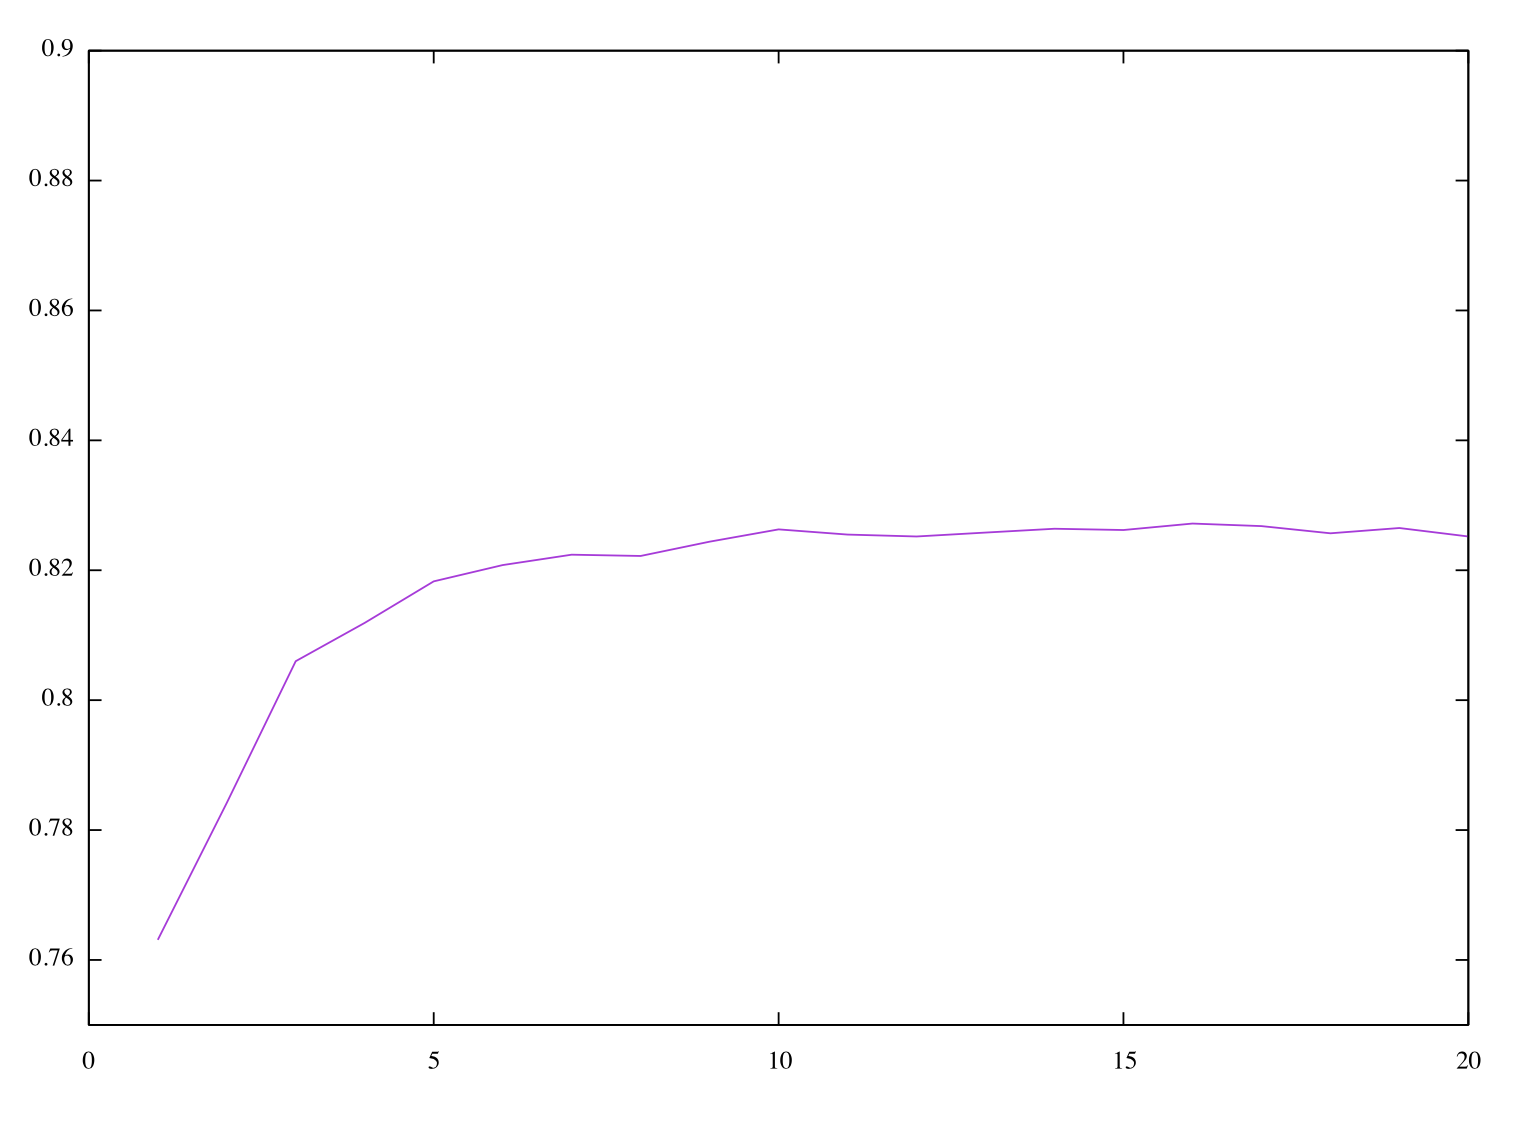
\includegraphics[scale = 0.5]{q62_plot.png}%
\label{fig:proto}%
\end{figure}

\section*{Part 3}
For the training of the LMNN model, I took 6K test points which were randomly selected from the given training set. I set the maxiter to 200,000. My model converged before the value reached 200,000. I got a test accuracy of 83.045\% for my model and with k=10 when I ran it on all the given 20K test points.

\end{mlsolution}
					
\end{document}